%\renewcommand{\ttdefault}{pcr}
%\lstset{basicstyle=\ttfamily}
%\lstset{framextopmargin=50pt,frame=bottomline}
%\lstset{language=C++}
%\begin{lstlisting}

%\begin{minted}{c++}
%GL_first_hmw.h
%#include <iostream>
%#include <math.h>
%#include <conio.h>

%using namespace std;

%//сравнения будем проводить с epsilon. Так как оно очень маленькое - то заменяем его в сравнении с нулем
%float epsilon=1.0e-7;

%void functionF();
%\end{minted}
%\end{lstlisting}

\begin{figure}[htbp]
    %\center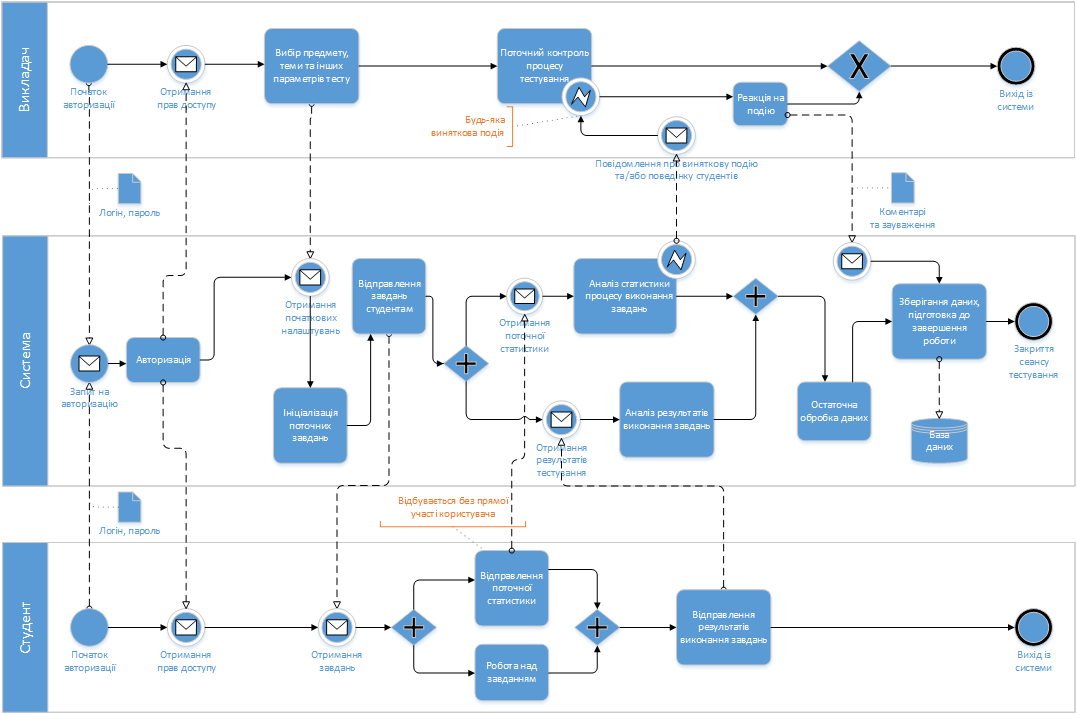
\includegraphics[height=23em,angle=90]{images/bpmn_tests.png}
    \center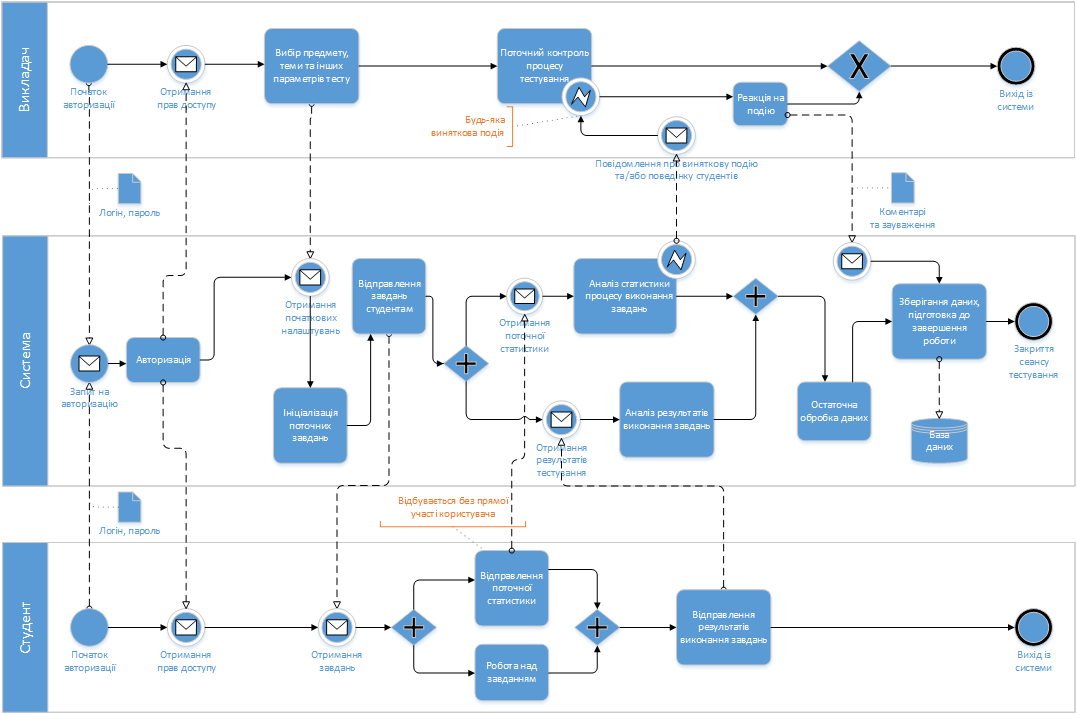
\includegraphics[width=\textwidth]{images/bpmn_tests.png}
    \caption{BPMN-діаграма процесу проміжної перевірки знань,
    побудована на базі підрозділу \ref{section:precedences}}
\end{figure}

\begin{figure}[htbp]
    \center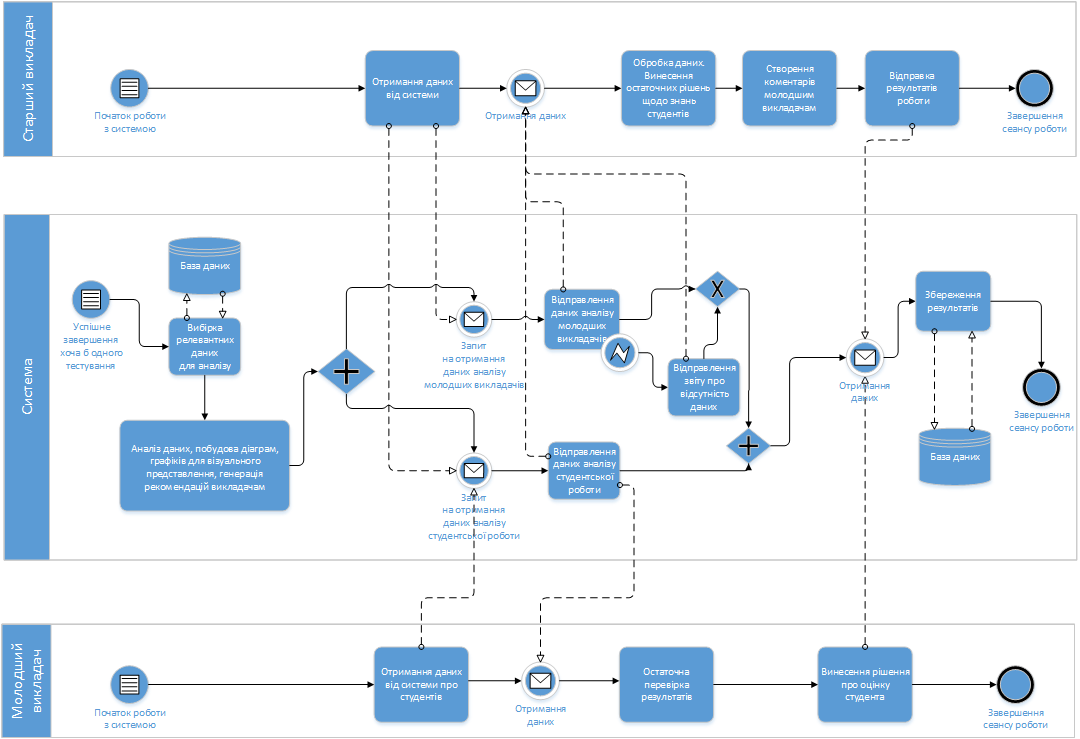
\includegraphics[height=33em,angle=90]{images/bpmn_teachers.png}
    \caption{BPMN-діаграма процесу взаємодії викладачів і системи}
\end{figure}
